%
%--- 
%-----------------------------------
\chapter{Results}
\label{ch:results}
%-----------------------------------
%---
% 

In order to validate our model, we simulate two nMOTs arrangements from different laboratories. One of them traps dysprosium atoms, whereas the other one traps strontium atoms. We choose experiments that perform nMOTs in the power-broadened regime. In this chapter, we shall present our simulated data and compare them with experimental measures.

% Dysprosium
%-----------------------------------
%
%-----------------------------------
\section{Dysprosium nMOT}
\label{sec:dysprosium-nMOT}
%-----------------------------------
%

We choose to simulate the dysprosium nMOT \cite{dreon2017optical} reproduced by Davide Dreon and his research group since it matches the conditions of our model and is thorough detailed in the Dreon PhD thesis \cite{dreon2017designing}, which is necessary to improve accuracy as discussed in section \ref{sec:input-outputs}.

\begin{wrapfigure}{l}{0.5\linewidth}
    \centering
    \caption{Electronic transitions of the dysprosium nMOT}
    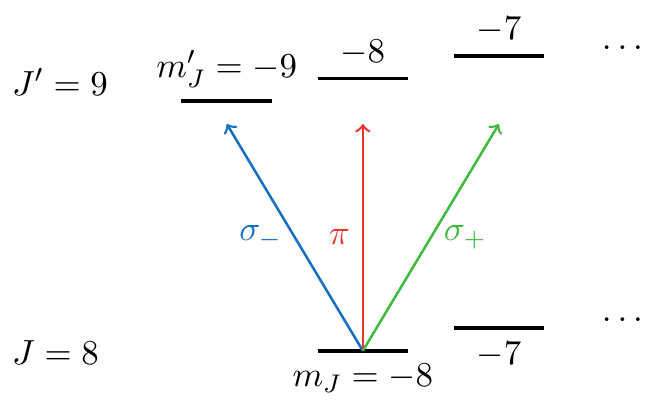
\includegraphics[width=0.45\textwidth]{USPSC-img/Dy-Dreon-transitions.png}
    \vspace{5px}
    \legend{. \\ Source: \cite{dreon2017optical}}
    \label{fig:Dy-Dreon-electronic-transitions}
\end{wrapfigure}
The involved electronic transition presented in table \ref{tab:electronic-transition-Dy-Dreon} yields a narrowness of $ \eta =  43.8 $ that is not small enough to reach the quantum regime, but it is enough to reach the power-broadened regime. Furthermore, in the presence of a magnetic field, the involved electronic transition $ J = 8 \longrightarrow J' = 9 $ has 36 possible states, which is much more complicated than the transition $ J = 0 \longrightarrow J = 1 $ presented in chapter \ref{ch:Monte-Carlo-simulation}. However, previous works \cite{lu2011strongly,aikawa2012bose} on nMOTs with Lanthanide atoms experimentally confirmed a spontaneous spin polarization that allows to simplify the transitions to $ \ket{J = 8, m_J = 8} \longrightarrow \ket{J' = 9, m_J' = -7, -8, -9} $ as  illustrated in figure \ref{fig:Dy-Dreon-electronic-transitions}.

\begin{table}[ht!]
    \centering
    \begin{tabular}{|c|c|c|}
        \hline
        \textbf{Symbol} & \textbf{Quantity} & \textbf{Value} \\ \hline
        $ \Gamma $ & Natural Linewidth & $ 2\pi \times 136\ kHz $ \\
        $ \lambda $ & Resonant wavelength & $ 626\ nm $ \\
        $ J_{gnd} $ & Ground state angular momentum & $ 8 $ \\
        $ g_{gnd} $ & Ground state Landè factor & $ 1.24 $ \\
        $ g_{exc} $ & Excited state Landè factor & $ 1.29 $ \\
        $ m $ & Mass & $ 164\ u $ \\
        \hline
    \end{tabular}
    \caption{Eletronic transition parameters of the dysprosium nMOT reproduced by \cite{dreon2017designing}.}
    \label{tab:electronic-transition-Dy-Dreon}
\end{table}

$ T_D = 3.26\ \mu K $

\begin{table}[ht!]
    \centering
    \begin{tabular}{|c|c|c|}
        \hline
        \textbf{Symbol} & \textbf{Quantity} & \textbf{Value} \\ \hline
        $ w $ & Waist & $ 2.0\ cm $ \\
        $ s_0 $ & Saturation parameter & $ 0.65 $ \\
        \hline
    \end{tabular}
    \caption{Laser setup features}
    \label{tab:lasers-setup}
\end{table}

\begin{table}[ht!]
    \centering
    \begin{tabular}{|c|c|c|}
        \hline
        \textbf{Symbol} & \textbf{Quantity} & \textbf{Value} \\ \hline
        $ B_0 $ & Axial gradient & $ 1.71 G $ \\
        $ B $ & Magnetic Field & $ B_0(-\hat{x} + \hat{y}/2 + \hat{z} / 2) $ \\
        $ B_{bias} $ & Bias & $ (-0.094 \hat{z})\ G / cm $ \\
        \hline
    \end{tabular}
    \caption{Magnetic quadrupole field}
    \label{tab:magnetic-field}
\end{table}

%-----------------------------------
\subsection{Atomic cloud profile}
\label{sec:cloud-profile-dysprosium}
%-----------------------------------

\begin{figure}[!ht]
    \centering
    \caption{Simulated ${}^{164}Dy$ cloud profile}
    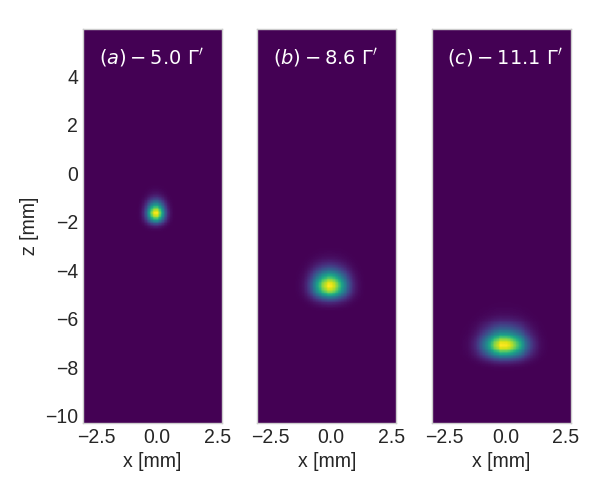
\includegraphics[width=0.7\textwidth]{USPSC-img/dy_dreon_cloud_profile.png}
    \vspace{5px}
    \legend{Simulated dysprosium cloud profile for three laser detunings: $ \delta = -5.0\Gamma' $ (a), $ \delta = -8.6\Gamma' $ (b), and $ \delta = -11.1\Gamma' $ (c), where $ \Gamma' = \Gamma \sqrt{1 + s_0} $ is the power-broadened linewidth. \\ Source: author}
    \label{fig:dy-atomic-cloud-profile}
\end{figure}

\begin{figure}[!ht]
    \centering
    \caption{Centre of mass of the ${}^{164}Dy$ nMOT}
    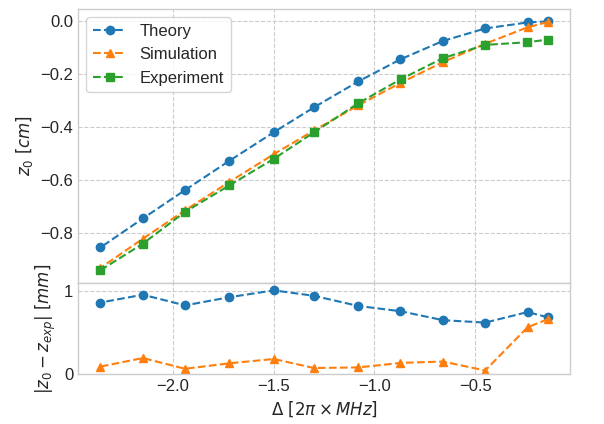
\includegraphics[width=0.7\textwidth]{USPSC-img/dy_centre_of_mass.png}
    \vspace{5px}
    \legend{centre of mass.\\ Source: author}
    \label{fig:dy-centre-of-mass}
\end{figure}

\begin{figure}[!ht]
    \centering
    \caption{Cloud size of the ${}^{164}Dy$ nMOT}
    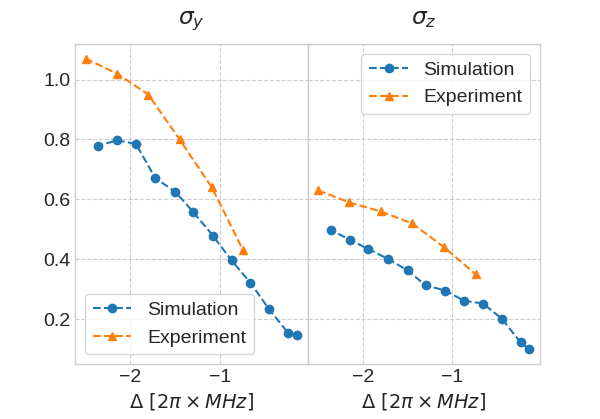
\includegraphics[width=0.7\textwidth]{USPSC-img/dy_cloud_size.png}
    \vspace{5px}
    \legend{cloud size.\\ Source: author}
    \label{fig:dy-cloud-size}
\end{figure}

\begin{figure}[!ht]
    \centering
    \caption{Cloud size ratio of the ${}^{164}Dy$ nMOT}
    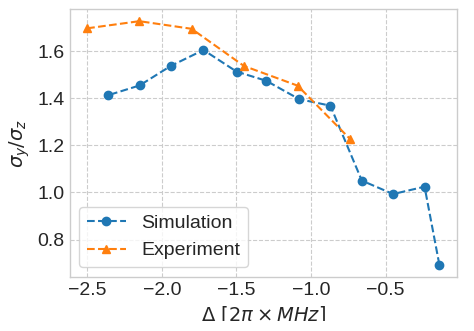
\includegraphics[width=0.55\textwidth]{USPSC-img/dy_cloud_size_ratio.png}
    \vspace{5px}
    \legend{cloud size ratio.\\ Source: author}
    \label{fig:dy-cloud-size-ratio}
\end{figure}

%-----------------------------------
\subsection{Temperature}
\label{temperature}
%-----------------------------------

\begin{figure}[!ht]
    \centering
    \caption{Temperature of the ${}^{164}Dy$ nMOT as a function of the laser detuning}
    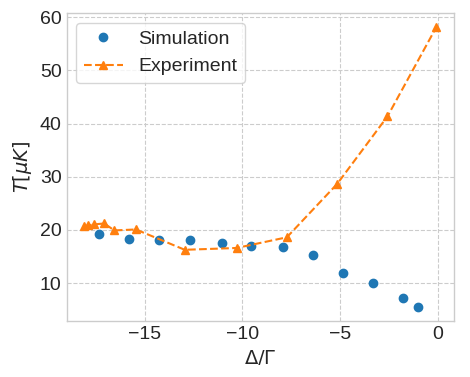
\includegraphics[width=0.6\textwidth]{USPSC-img/dy_temperature.png}
    \vspace{5px}
    \legend{temperature.\\ Source: author}
    \label{fig:dy-temperature}
\end{figure}

%-----------------------------------
%

% Strontium
%-----------------------------------
%
%-----------------------------------
\section{Strontium}
\label{eq:strontium}
%-----------------------------------
%

We shall simulate two strontium nMOTs reproduced at different laboratories. The first one, which we call \textbf{strontium-ifsc}, is managed by the research group of the professors Philippe W. Courteille at São Carlos Institute of Physics and Raul C. Teixeira at the Federal University of São Carlos. The second one, which we call \textbf{strontium-loftus}, is reported in the paper \cite{loftus2004narrow} and is one of the main references for nMOTs.

%-----------------------------------
\subsection{Atomic cloud profile}
\label{sec:cloud-profile-dysprosium}
%-----------------------------------

Experimental data from the \textit{strontium-loftus}.

\begin{figure}[!ht]
    \centering
    \caption{Simulated ${}^{88}Sr$ cloud profile}
    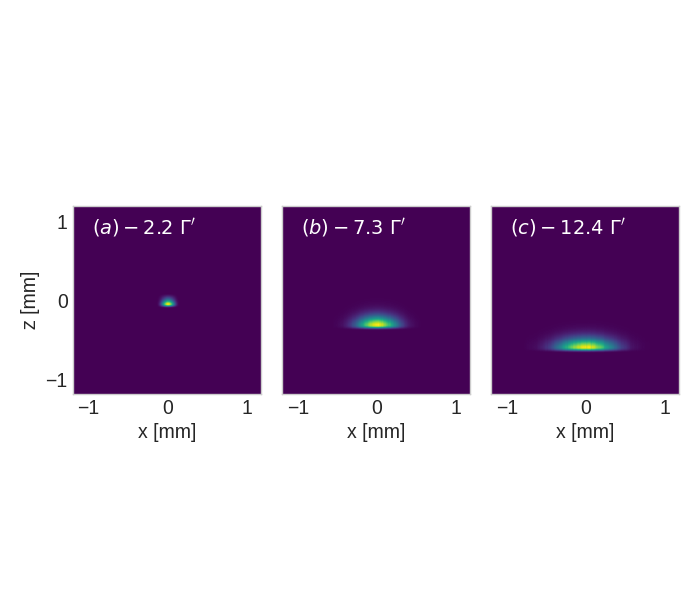
\includegraphics[width=0.9\textwidth]{USPSC-img/sr_loftus_cloud_profile.png}
    \vspace{5px}
    \legend{Simulated strontium cloud profile for three laser detunings: $ \delta = -5.0\Gamma' $ (a), $ \delta = -8.6\Gamma' $ (b), and $ \delta = -11.1\Gamma' $ (c), where $ \Gamma' = \Gamma \sqrt{1 + s_0} $ is the power-broadened linewidth. \\ Source: author}
    \label{fig:sr-loftus-atomic-cloud-profile}
\end{figure}

\begin{figure}[!ht]
    \centering
    \caption{Centre of mass of the ${}^{88}Sr$ nMOT as a function of the lasers detuning}
    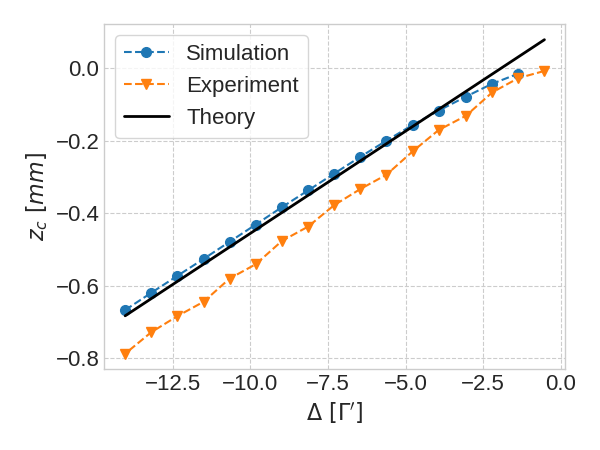
\includegraphics[width=0.6\textwidth]{USPSC-img/sr_centre_of_mass.png}
    \vspace{5px}
    \legend{centre of mass.\\ Source: author}
    \label{fig:sr-centre-of-mass}
\end{figure}

\begin{figure}[!ht]
    \centering
    \caption{Cloud size of the ${}^{88}Sr$ nMOT}
    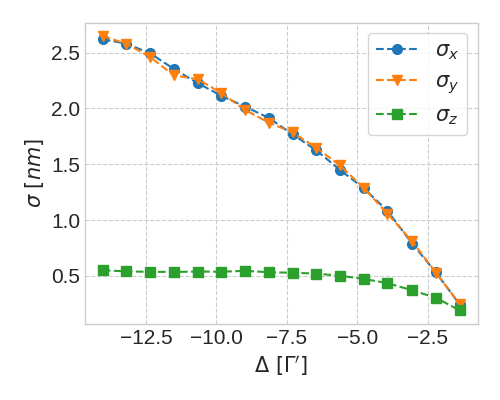
\includegraphics[width=0.8\textwidth]{USPSC-img/sr_loftus_cloud_size.png}
    \vspace{5px}
    \legend{cloud size.\\ Source: author}
    \label{fig:sr-loftus-cloud-size}
\end{figure}


%-----------------------------------
\subsection{Temperature}
\label{temperature}
%-----------------------------------

Experimental data from the \textit{strontium-ifsc}.

\begin{figure}[!ht]
    \centering
    \caption{Temperature of the ${}^{88}Sr$ nMOT as a function of the lasers detuning}
    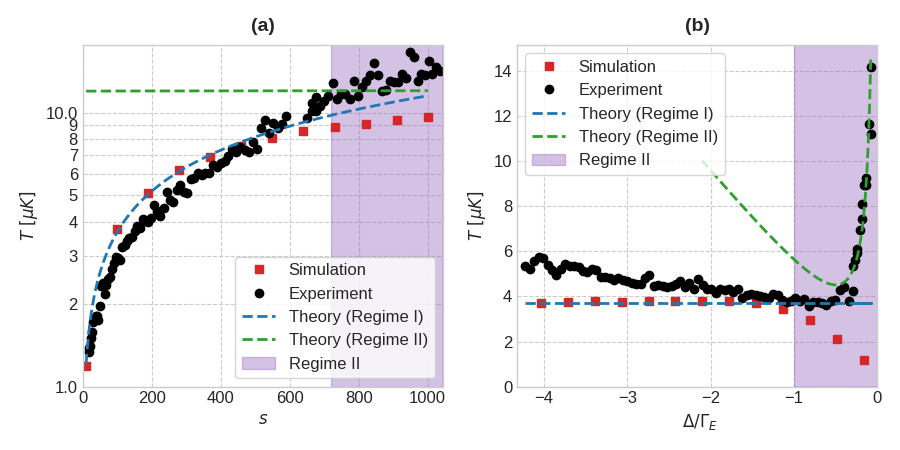
\includegraphics[width=1.0\textwidth]{USPSC-img/sr_temperature.png}
    \vspace{5px}
    \legend{temperature.\\ Source: author}
    \label{fig:sr-temperature}
\end{figure}

%-----------------------------------
%
